\chapter{Die Konsolen Applikation}
\label{cha:the-console-app}
Da in dieser Arbeit das Design der bestehenden Implementierung diskutiert und ein Designvorschlag eingebracht werden soll, muss man zuerst die Struktur und das Design der bestehenden Implementierung verstehen lernen. Da sich die meiste Geschäftslogik in der Konsolen Applikation befindet wird im folgenden dessen Design und Struktur diskutiert.\\

\begin{figure}[h]
\centering
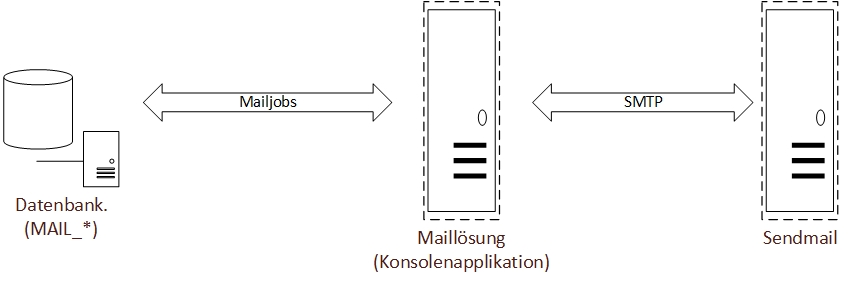
\includegraphics[scale=0.5]{systemaufbau_console_alone.jpg} 
\caption{Teilsystem Konsolen Applikation und Sendmail}
\label{fig:class-hierarchie-email}
\end{figure}


\newpage
\section{Klassenhierarchie}
\label{sec:console-app-class-hierarchie}
Um die Struktur der Konsolen Applikation  zu verstehen wenden wir uns den implementierten Klassenhierarchien der einzelnen Softwarekomponenten wie E-Mail Typen und DAOs (Datenzugriffsobjekte) zu. Diese beiden Softwarekomponenten stellen den Hauptteil der Software dar, daher beginnen wir mit der Analyse dieser Komponenten. 
\subsection{E-Mail Typen}
Einleitend betrachten wir die implementierte Klassenhierarchie der E-Mail Typen mit einem Ausschnitt aus der Klassenhierarchie. Dieser Ausschnitt illustriert sehr gut die vorhandene Struktur der Klassenhierarchie.
\begin{figure}[h]
\centering
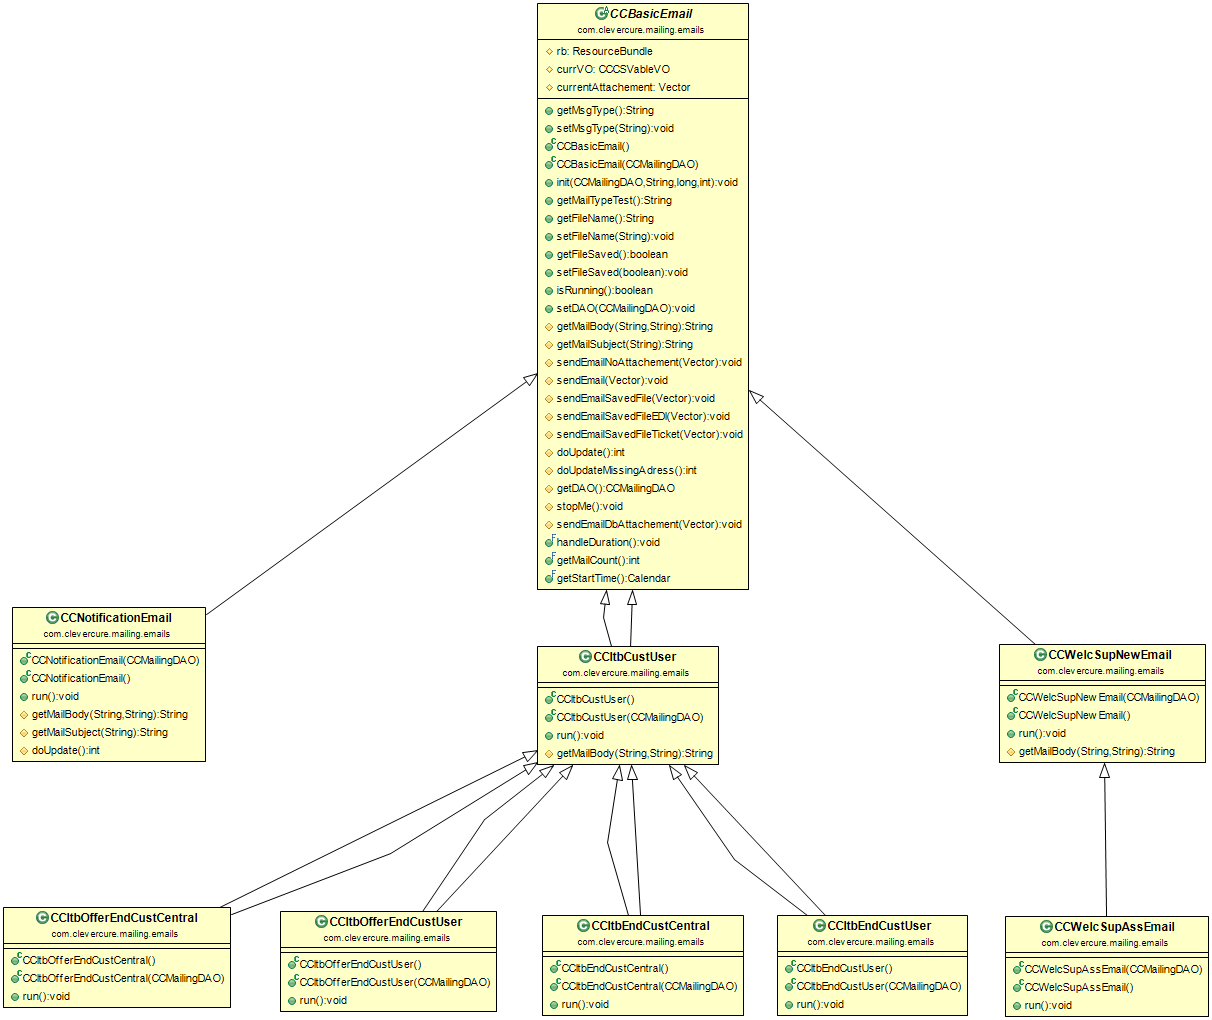
\includegraphics[scale=0.35]{class_diagram_basic_email.png} 
\caption{Die Basisklasse \emph{BasicEmail} mit einigen Implementierungen}
\label{fig:class-hierarchie-email}
\end{figure}

\newpage
Man hat sich hier für das \emph{Factory Method Muster} entschieden wobei die Basisklasse \emph{BasicEmail} eingeführt wurde, welche die gesamte Logik für den Aufbau und Versand einer E-Mail in sich kapselt und die einzelnen konkreten Implementierungen, in Form von abgeleiteten Klassen, die die einzelnen E-Mail Typen darstellen. Wie im Diagramm bei der Klasse \emph{CCItbCustUser} ersichtlich wurden auch E-Mail Typen implementiert, die ihrerseits wieder als Basisklasse dienen für untergeordnete E-Mail Typen. Aufgrund des vergebenen Namens kann man annehmen dass es sich hier um E-Mail Benachrichtigungen für einen Benutzer eines Kunden des Moduls ITB handelt, die man versucht hat zu gruppieren.\\
Die Gruppierung wurde hier durch Einführung einer eigenen Vererbungshierarchie auf Basis einer eingeführten Basisklasse \emph{CCItbCustUser}, die ihrerseits die eigentliche Basisklasse \emph{BasicEmail} weg abstrahiert, realisiert.\\

An sich ist dies kein schlechter Ansatz jedoch erwarte ich mir von einer konkreten Implementierung, dass diese auch ein gewisses Maß an Logik beinhaltet, die das Factory-Method Muster rechtfertigt, jedoch ist dies in den meisten Fällen nicht der Fall. Solche Klassenhierarchien einzuführen nur um verschiedene Datentypen zu erhalten, welche einen E-Mail Typ definieren, welcher nicht einmal in den angeschlossenen Systemen verwendet wird sondern nur innerhalb dieser Konsolen Applikation finde ich übertrieben. Es gibt weitaus einfachere, weniger aufwendige und Code produzierende Ansätze mit denen E-Mail Typen abgebildet werden können.

\newpage
\subsection{Datenzugriffsobjekt(e)}
Nachdem wir die Klassenhierarchie der E-Mail Typen analysiert haben wenden wir uns nun der Datenbankzugriffsschicht zu, die mit einem einzigen DAO (Datenzugriffsobjekt) implementiert wurde.
\begin{figure}[h]
\centering
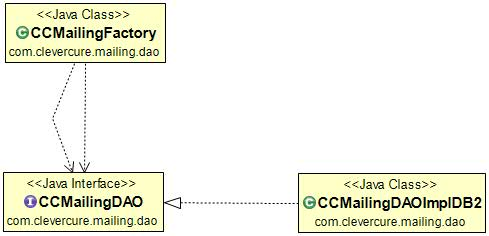
\includegraphics[scale=0.5]{cc_mail_dao.jpg} 
\caption{Die \emph{CCMailingDAOImplDB2} Implementierung mit seinem Interface \emph{CCMailingDAO} mit seiner Factory \emph{CCMailingFactory}}
\label{fig:class-hierarchie-email}
\end{figure}
\ \\
Obwohl man eine Klassenhierarchie für die E-Mail Typen eingeführt hat, hat man dies bei den DAOs (Datenzugriffsobjekte) nicht getan. Es gibt also eine einzige DAO Implementierung, die alle Datenbankabfragen über alle E-Mail Typen hinweg beinhaltet und diese über eindeutige Methodennamen identifiziert. Des Weiteren wurde zwar eine Factory für dieses DAO eingeführt, aber eine Factory für ein DAO mit \emph{Class.forName("*.DaoImplDb2")} erscheint fast sinnlos, obwohl man hier noch die Begründung finden könnte, dass diese Factory eingeführt wurde um zumindest die konkrete Datenbank zu abstrahieren und die Möglichkeit zu schaffen die DAO Implementierung für DB2 auf z.B.: Oracle zu ändern. Man würde hier erwarten das die DAO Implementierungen kontextabhängig - also auf Modulebene - implementiert worden wären und dass die Factory dynamisch mit der zu verwendenden Implementierung initialisiert werden kann, also parametriebar ist. Dann wäre es aber auch erforderlich die Datenbank spezifischen Implementierungen über ein eigenes Artifakt zur Verfügung zu stellen und nicht das alle Ressourcen sich innerhalb ein und desselben Artifaktes befinden, also die Interface Spezifikationen und dessen Implementierungen.

\newpage
\section{Implementierung}
Da wir nun die Klassenhierarchien kennen gelernt haben wenden wir uns deren Implementierung zu. Im folgenden werden die Implementierungen der Klasse \emph{CCItbCustUser} und dessen Ableitungen diskutiert. Im Punkt~\ref{sec:console-app-class-hierarchie} wurde behauptet dass diese Ableitungen eingeführt wurden um E-Mail Typen zu gruppieren. Man könnte aber auch davon ausgehen dass diese eigene Vererbungshierarchie eingeführt wurde um Funktionalitäten für die einzelnen E-Mails zu kapseln. Analysieren wir nun diese Implementierungen um zu sehen welche Funktionalitäten in einen E-Mail Typ implementiert wurden. \\\\
Die folgende Implementierung dient als Beispiel für eine Implementierung eines E-Mail Typs.   

\begin{program}
\caption{CCItbCustUser E-Mail Typ Implementierung}
\label{CCItbCustUser.java}
\begin{JavaCode}
public class CCItbCustUser extends CCBasicEmail {
	
	private Map cache = new HashMap();

	public CCItbCustUser() {
		super();
	}

	public CCItbCustUser(CCMailingDAO dao) {
		super(dao);
	}

	@Override
	String getMailType() {
		return "ISCU";
	}
	
	@Override
	public void run() {
		try {
			sendEmailNoAttachement(getDAO().getItbStartCustUserMailText());
		} catch (DAOSysException ex) {
			LOG.error("DAOSysException in CCItbCustUser.run: ",
						ex);
		} finally {
			stopMe();
		}
	}
	
	@Override
	protected String getMailBody(String bodyKey, String bodySQLKey)
		throws DAOSysException {
		int lanId = ((CCItbVO)currVO).getLanguageId();
		int itbhId = ((CCItbVO)currVO).getItbhID();
		String body = "";
		String key = itbhId	+ "_" + lanId;
		if (cache.containsKey(key)) {
			body = (String) cache.get(key);
			LOG.debug("48: Got from cache key: " + key 
								+ " body: " + body);
		} else {
			Object [] allParams = getDAO().getItbCustData((CCItbVO)currVO, 19);
			// Message body parameters retrieved from result set for body template
			MessageFormat form = new MessageFormat(rb.getString(bodyKey).trim());
	 		body = form.format(params);
	 		cache.put(key, body);
	 		LOG.debug("48: DB access for the key: " + key
	 						+ " got body: " + body);
		}
		return body;
	}
}
\end{JavaCode}
\end{program}

\newpage
In dieser Implementierung ist gut zu erkennen, dass die einzelnen E-Mail Typen - oder mit anderen Worten - die einzelnen Implementierungen der Basisklasse \emph{BasicEmail} lediglich folgende Funktionalitäten implementieren:
\begin{itemize}
	\item\emph{getMailType()}\\
	Bereitstellen eines eindeutigen Schlüssels, der diesen E-Mail Typ identifiziert.
	\item\emph{getMailBody()}\\
	Erstellen der E-Mail Nachricht aus einer Vorlage, welche mit Parametern - Daten werden aus Datenbank gelesen - befüllt wird.
	\item\emph{run()\\}
	Einstiegspunkt des E-Mail Typs, wo definiert wird welche Art von E-Mail erstellt werden soll. (\emph{BasicEmail} stellt mehrere Methoden zur Verfügung)
\end{itemize}
\ \\

\chapter{Client Implementierung}
\label{cha:client-api}
Da die Kommunikation ausschließlich über die Datenbank erfolgt ist eine echte Client API nicht vorhanden. Alle Systeme implementieren das Erstellen der Mailjob Einträge selbstständig und es wird keine gemeinsame Client API verwendet, was einen gewissen Grad der Inkonsistenz bei Änderungen der Datenstruktur sowie der Semantik der Daten mit sich bringt. Als Beispiel wird hier die Semantik der einzelnen Spalten angeführt, die zwar technisch sich innerhalb einer Datentyp Domain befinden, sich die semantische Bedeutung der enthaltenen Daten aber unterscheidet. Dies ist zwar Teil der Datenbank Integration aber die Tatsache dass diese Semantik rein innerhalb der Applikation abgebildet werden kann und nicht über die Datenbankfunktionalitäten wie z.B.: Fremdschlüssel wird dieser Teil hier diskutiert. Da die Maillösung über SQL Abfragen die Daten für die E-Mail Nachricht erhält müssen auch Parameter bereitgestellt werden, die in der SQL Abfrage gesetzt werden. Diese Parameter wurden \emph{'generisch'} über eine festgesetzte Anzahl von Tabellenspalten abgebildet, dessen enthaltene Daten je nach E-Mailtyp anders interpretiert werden. Es kann also sein das ein Eintrag einer Tabellen für die Spalte \emph{COL\_1} einen String enthält mit dem Wert \emph{'Thomas Herzog'} und ein anderer Eintrag einen string mit dem Wert \emph{'14'} der in der SQL Abfrage aber als Integer Datentyp behandelt wird. Die Systeme die Mailjobs erzeugen müssen sich also dem Kontext einer E-Mail bewusst sein, sowie müssen berücksichtigen, dass die richten Spalten der Tabelle \emph{MAIL\_JOB} mit den richtigen Daten befüllt werden, wobei auch beachtet werden muss in welchen Datentyp der Datensatz in weiterer Folge durch die Mailösung interpretiert wird.\\
Dies ist in meinen Augen sehr inkonsistent und fehleranfällig und hat auch schon einige Probleme verursacht.\\\\
\begin{figure}[h]
\centering
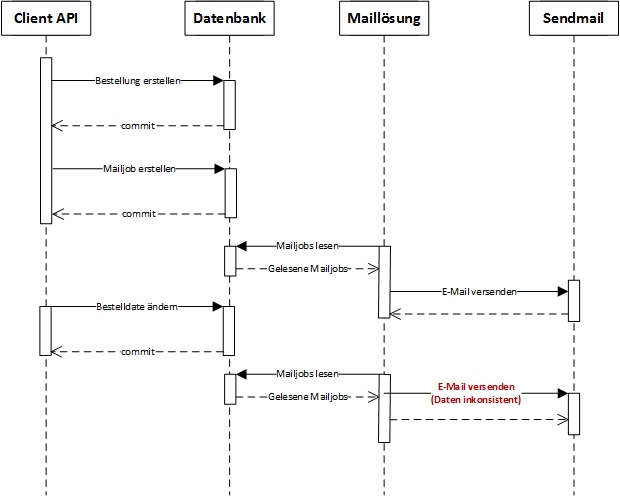
\includegraphics[scale=0.70]{Emailvesand_Client_Api.jpg}
\caption{Diese Abbildung zeigt das Problem der inkonsistenten Daten beim erneuten E-Mailversand einer bereits versendeten E-Mail, mit dem Beispiel einer angelegten und anschließend geänderten Bestellung, auf}
\label{fig:sequence-diagram-mail-send}
\end{figure}
\newpage
